% Consumer surplus under a linear demand curve.
% Compile to SVG:  latex consumer_surplus.tex && dvisvgm --no-fonts consumer_surplus.dvi -o ../consumer_surplus.svg
\documentclass[tikz,border=6pt]{standalone}
\usepackage[scaled]{helvet}
\renewcommand{\familydefault}{\sfdefault}
\usetikzlibrary{arrows.meta}
\definecolor{yel}{HTML}{F2C94C}
\definecolor{grn}{HTML}{8FC98F}
\begin{document}
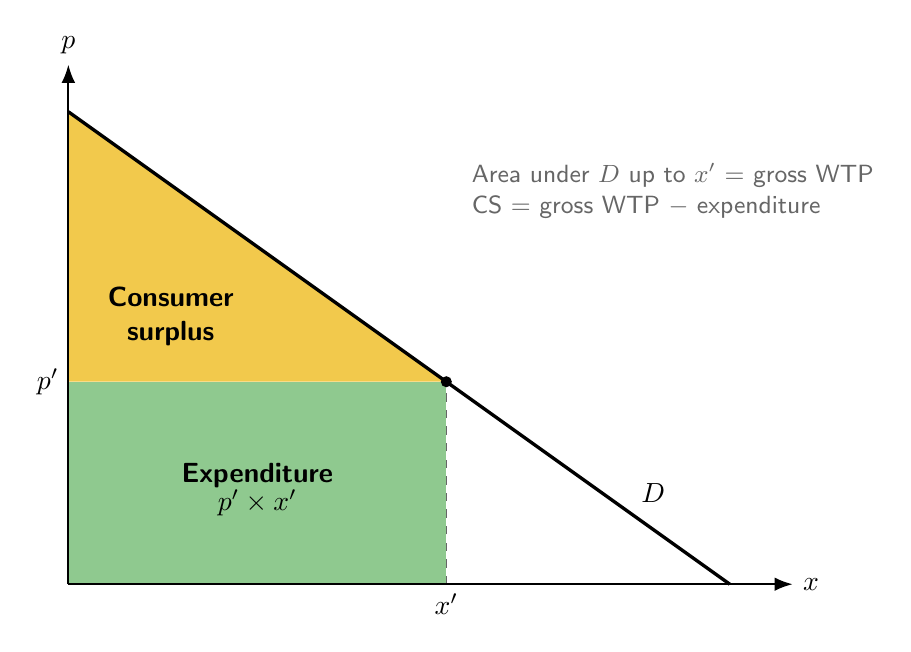
\begin{tikzpicture}[scale=1]
  % demand: p = 10 - (10/14) x ; purchase at x' = 8 -> p' = 4.29
  \def\xs{8}
  \pgfmathsetmacro{\ps}{10 - 10/14*\xs}
  \fill[yel] (0,10*0.6) -- (0,\ps*0.6) -- (\xs*0.6,\ps*0.6) -- cycle;
  \fill[grn] (0,0) rectangle (\xs*0.6,\ps*0.6);
  \draw[dashed, black!60] (\xs*0.6,0) -- (\xs*0.6,\ps*0.6);
  \draw[very thick] (0,6) -- (14*0.6,0) node[pos=0.85, above right] {$D$};
  \fill (\xs*0.6,\ps*0.6) circle (2pt);
  \draw[-{Latex}, thick] (0,0) -- (9.2,0) node[right] {$x$};
  \draw[-{Latex}, thick] (0,0) -- (0,6.6) node[above] {$p$};
  \node[left]  at (0,\ps*0.6) {$p'$};
  \node[below] at (\xs*0.6,0) {$x'$};
  \node[font=\bfseries, align=center] at (1.3,3.4) {Consumer\\surplus};
  \node[font=\bfseries, align=center] at (2.4,1.2) {Expenditure\\[-2pt]\normalfont $p'\times x'$};
  \node[black!60, font=\small, align=left, anchor=west] at (5,5)
     {Area under $D$ up to $x'$ = gross WTP\\CS = gross WTP $-$ expenditure};
\end{tikzpicture}
\end{document}
